% TEMPLATE WHICH I USE FOR ALL MY UNIVERSITY ASSIGNMENTS INCLUDING THE PROJECT 1 SUBMISSION

\documentclass[a4paper]{article}
\usepackage[utf8]{inputenc}
\usepackage{draculatheme}
\usepackage{graphicx}
\usepackage{color}
\usepackage{nopageno}
\usepackage{fontawesome}
\usepackage{listings}
\usepackage[export]{adjustbox}
\usepackage[fontsize=8pt]{fontsize}

\usepackage[a4paper, total={7.8in, 11.5in}]{geometry}
\graphicspath{ {./images/} }
\title{Project 2 Submission}
\author{Chaitanya Sharma}
\date{January 2023}

\makeatletter
\renewenvironment{abstract}{%
    \if@twocolumn
    \section*{\abstractname}%
    \else
    \begin{center}%
    {\bfseries \Large\abstractname\vspace{\z@}}
    \end{center}%
    \quotation
    \fi}
    {\if@twocolumn\else\endquotation\fi}
\makeatother
\begin{document}
    \begin{center}
        \begin{abstract}
            This is the design document of Chaitanya Sharma for Project 2 for ECE 250's Winter 2023 offering.
        \end{abstract}
    \end{center}


    \section{Introduction}
    My program consisted of a base abstract class {\color{draculapurple}HashPageTable}, and two derived classes ,namely {\color{draculapurple}OpenAddressedTable} and
        {\color{draculapurple}SeparateChainedTable} with dynamic array class for Chaining called {\color{draculapurple}DynamicArrayForProcess}.
    Also, according to the first word in the test case, the {\color{draculapurple}main} function calls
    either of {\color{draculapurple}OpenAddressedTableDriver} or {\color{draculapurple}ChainedTableDriver} for which I follow the
    parsing designs given by the ECE 250 staff.
    I have three {\color{Awesome}GLOBAL VALUES} defined,
    which act as placeholders for empty and deleted values, there values are {\color{LimeGreen}EMPTY\_PID}$=0$,
        {\color{LimeGreen}NULL\_MSTART}$=UINT\_MAX=4294967295$ and {\color{LimeGreen}TOMBSTONE\_PID}$=UINT\_MAX=4294967295$.
    \newline I've tested all edge test cases possible and also used the test cases provided by the
    jekelautograder on {\color{DarkPastelBlue}https://github.com/JZJisawesome/ece250-testcases}.
    \newline
    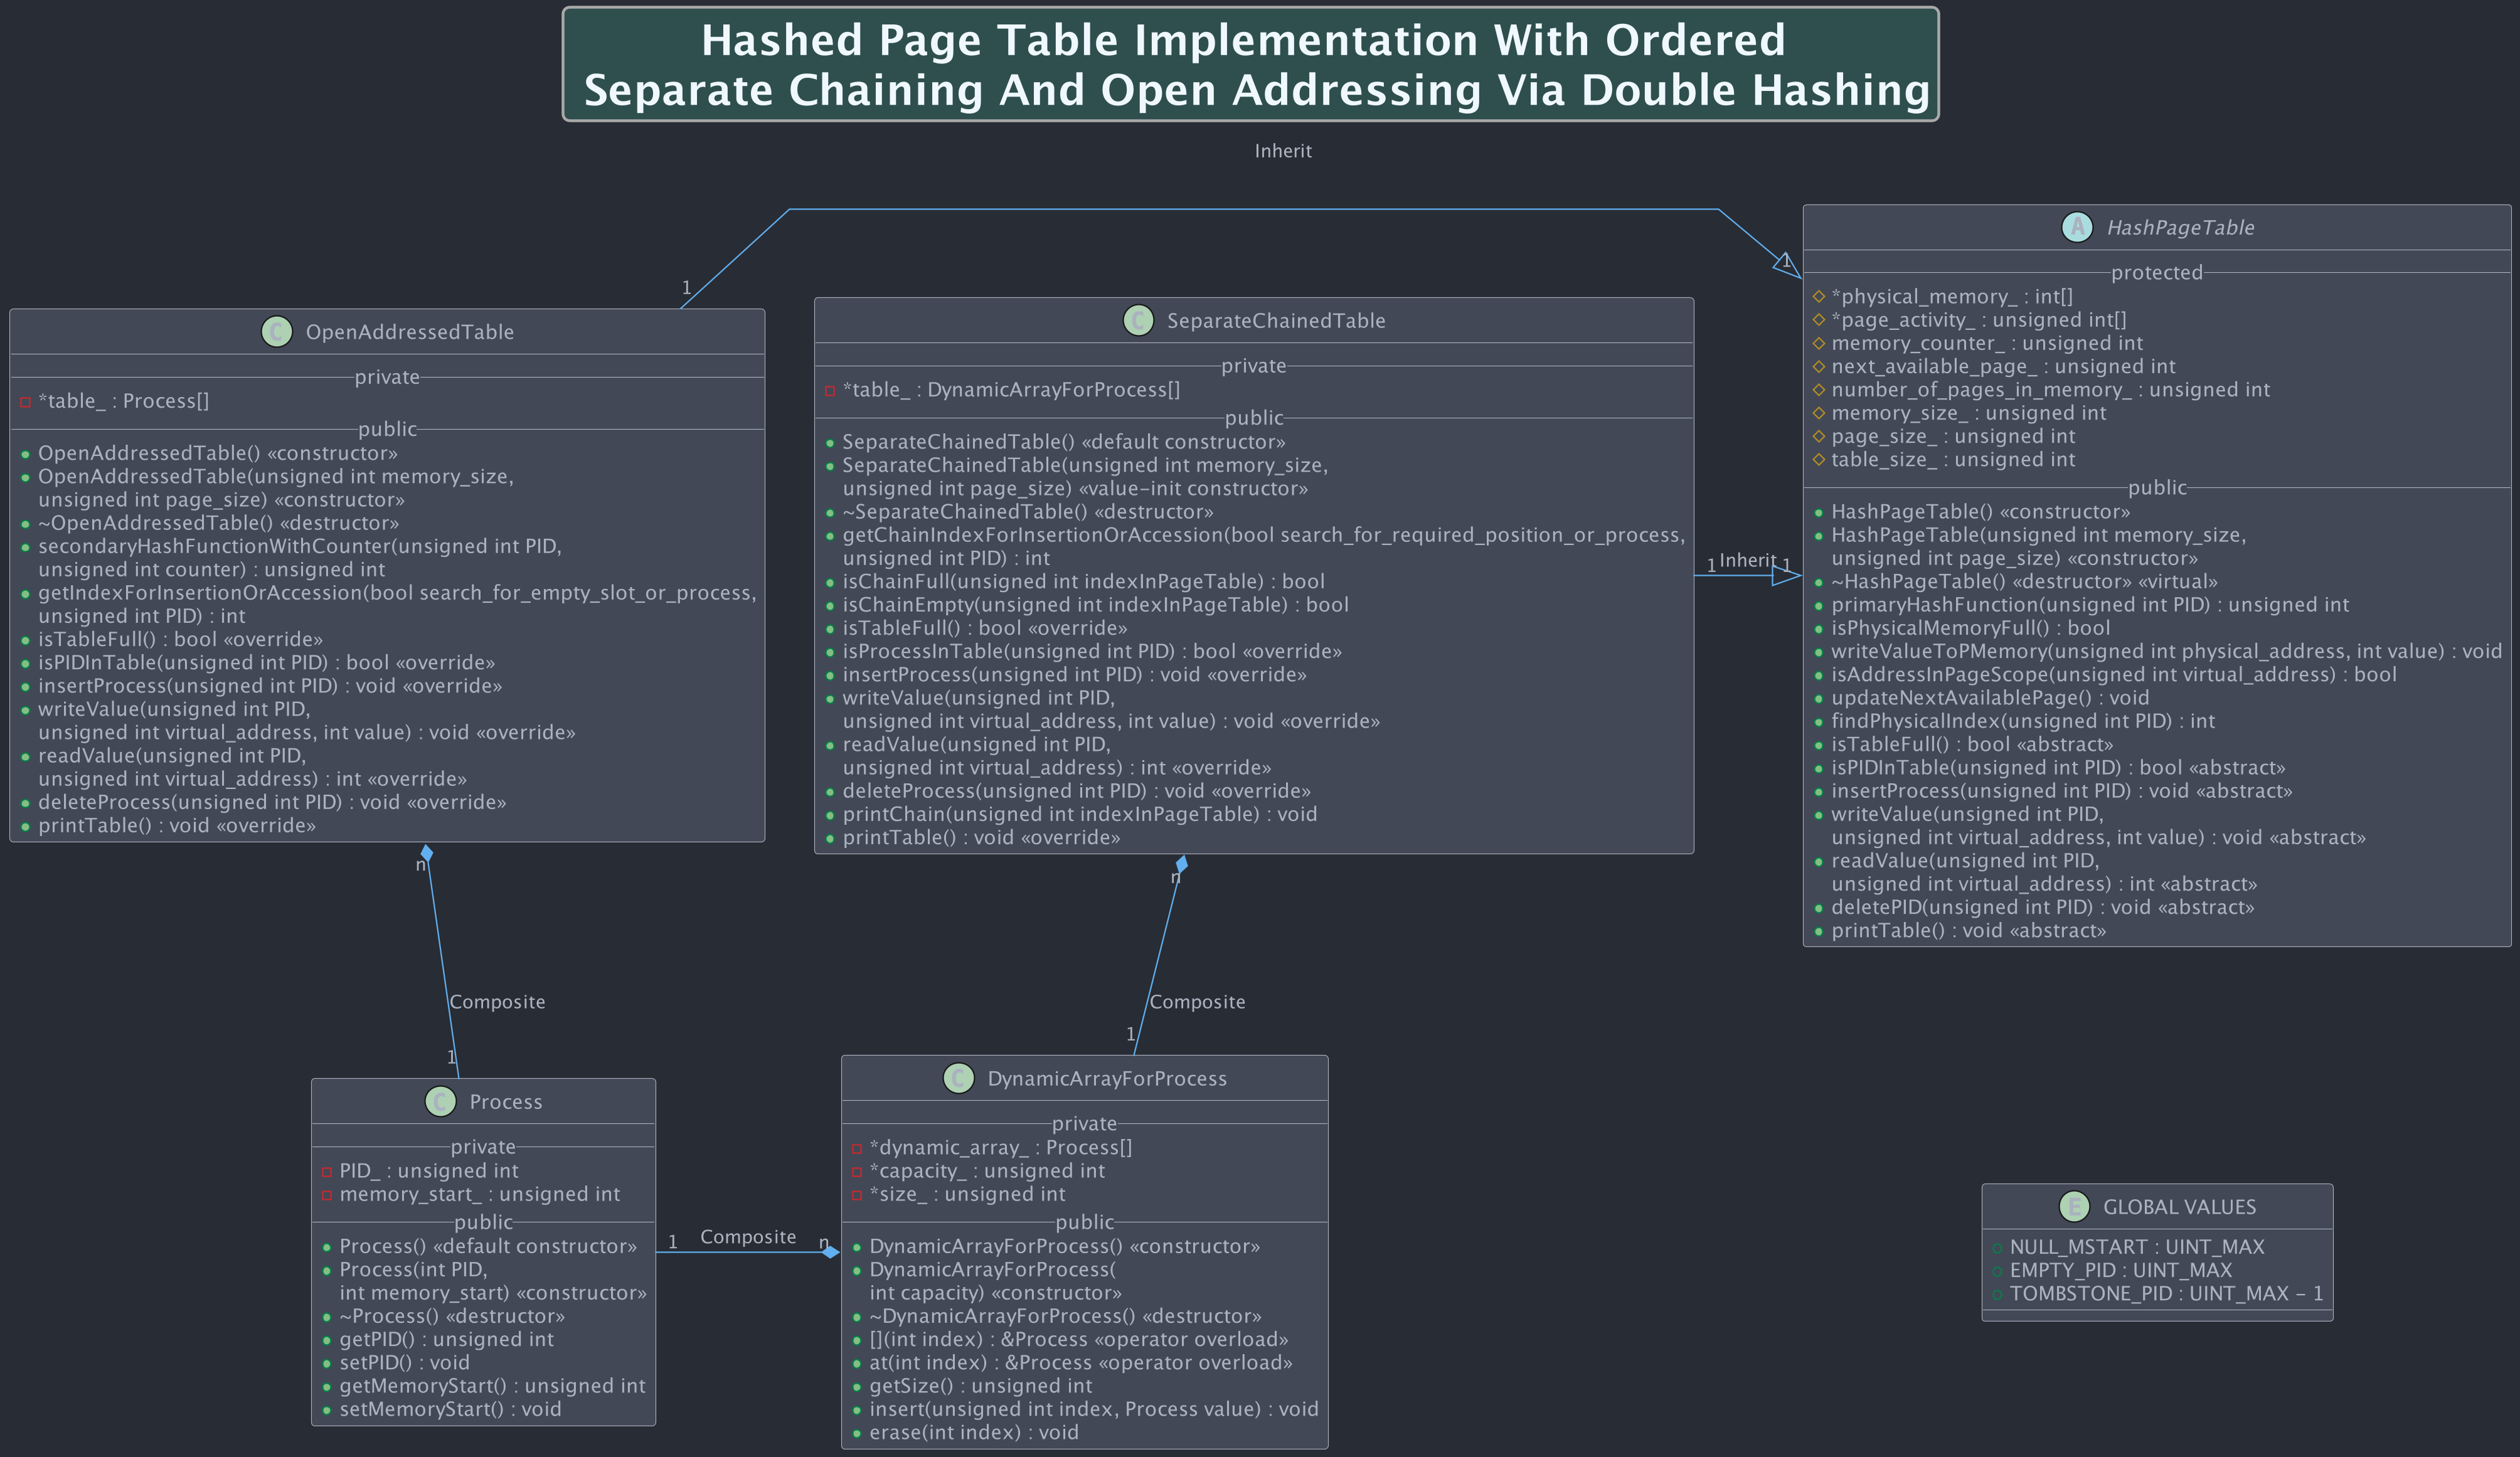
\includegraphics[scale=0.145, center]{PageTable.png}


    \section{Class Structure}

    \subsection{{\color{orange}class} {\color{draculapurple}Process}}
    This is a very simple class which only holds two pieces of information, the {\color{Turquoise}PID\_} and the
        {\color{Turquoise}memory\_start\_}, and I've provided the appropriate {\color{draculapurple}constructors()}, a
        {\color{draculapurple}default destructor()} and getters and setters for the two variables. The {\color{Turquoise}memory\_start\_} is
    like a virtual pointer to an index(or address) in the physical memory. And in the abstract design,
    two processes should neither ever have the same {\color{Turquoise}PID\_} or the same {\color{Turquoise}memory\_start\_},
    except when they're deleted or initialized to by the default constructor which would give them the value of
        {\color{LimeGreen}TOMBSTONE\_PID} or {\color{LimeGreen}EMPTY\_PID} respectively and a memory start of
        {\color{LimeGreen}NULL\_MSTART}.

    \subsection{{\color{orange}class} {\color{draculapurple}HashPageTable}}
    In this class most of the functions are actually pure virtual functions, except the {\color{draculapurple}constructor()}, {\color{draculapurple}destructor()},
    status boolean helper functions like {\color{draculapurple}isPhysicalMemoryFull}, the helper functions which deal with the
    physical memory like {\color{draculapurple}findPhysicalIndex{}} and obviously the {\color{draculapurple}primaryHashFunction()}.
    I've allocated all types of data structures which I would need, but aren't unique to the derived classes, in this class like the
        {\color{Turquoise}physical\_memory\_[]}, {\color{Turquoise}page\_activity\_[]} and more. I've used the {\color{Turquoise}page\_activity\_[]}
    to keep track of the statuses of each page in physical memory, and used a virtual pointer called {\color{Turquoise}next\_available\_page\_} which I update using {\color{draculapurple}updateNextAvailablePage()}.
    I'll explain all other logic since they're unique to the derived classes. The runtime of all functions defined in this class are {\color{lightblue}O(1)} since they all just use the
        {\color{draculapurple}primaryHashFunction()} to their operations, and the {\color{draculapurple}primaryHashFunction()} is {\color{lightblue}O(1)},
    and the {\color{draculapurple}updateNextAvailablePage()} is dependant on the hash function, so due to our assumption of even spread, it is also {\color{lightblue}O(1)}.

    For the destructor, I delete all appropriate dynamically allocated objects and equal them to {\color{LightPink}nullptr}.

    \subsection{{\color{orange}class} {\color{draculapurple}DynamicArrayForProcess}}
    Instead of using the bloated {\color{draculapurple}std::vector} class, I've created my own dynamic array class
    which is dynamically allocated process array, and for it's design, I've taken inspiration from the actual
        {\color{draculapurple}std::vector} class, and I've used the same logic for the {\color{draculapurple}DynamicArrayForProcess} class.
    Since I would only be using the functions {\color{draculapurple}insert()}, {\color{draculapurple}erase()},
        {\color{draculapurple}size()} and the appropriate operators overloads {\color{draculapurple}operator[]} and {\color{draculapurple}at},
    I've only implemented those functions. When referring to {\color{draculapurple}std::vector} class, as "bloated", I mean that
    for the purpose of a Page Table, most of its functionalities would be useless, and hence I've created my own class.
    Since even when using {\color{draculapurple}std::vector}, we were assuming the insertion, deletion and copy
    operations(for increasing size), we were assuming the runtime of the functonalities to be insignifigant, inside the concept of Hashing.
    Hence, the runtime of all the functions in this class are {\color{lightblue}O(n)} but considered {\color{lightblue}O(1)} for the
    abstraction purpose of this project. This class will produce an aggregation object of the {\color{draculapurple}Process} class's objects.

    For the destructor, I delete all appropriate dynamically allocated objects.

    \subsection{{\color{orange}class} {\color{draculapurple}SeparateChainedTable}}

    The main component of this class is a pointer which when initialized properly is an a dynamic array object of type

        {\color{draculapurple}DynamicArrayForProcess} with the size {\color{lightblue}$\frac{N(memory\ size)}{P(page\ size)}$}. Hence, it essentially acts as a 2D array.
    Since the {\color{draculapurple}DynamicArrayForProcess} object itself initializes without an element and resizes
    according to need, I do not initialize the internal index {\color{draculapurple}DynamicArrayForProcess} objects with a specified size.
    In this class, I have an empty constructor which just calls the empty {\color{draculapurple}constructor()} of the {\color{draculapurple}HashPageTable} class and
    initializes {\color{Turquoise}table\_} to {\color{LightPink}nullptr} , a value-init {\color{draculapurple}constructor()},
    which calls the value-init {\color{draculapurple}constructor()}, but at the same time, initializes the {\color{Turquoise}table\_} with the value
        {\color{lightblue}$\frac{N}{P}$}.

    For the destructor, I delete all appropriate dynamically allocated objects as well as call the destructor of the {\color{draculapurple}HashPageTable} class.

    Then there are chain status boolean functions like {\color{draculapurple}isChainEmpty()} and
        {\color{draculapurple}isChainFull()} whose names are self-descriptive, and functions like
        {\color{draculapurple}isTableFull()} and {\color{draculapurple}isProcessInTable()} which returns boolean values.

    \subsubsection{{\color{orange}int} {\color{draculapurple}getChainIndexForInsertionOrAccession}( {\color{orange}bool} search\_for\_required\_position\_or\_process, {\color{orange}unsigned int} PID)
        \faStar~~{\color{Awesome}a special feature of my code}~~\faStar}
    I call this function a double option finder function, as function serves two purposes, one for insertion and one for accession, decided by the {\color{orange}bool} parameter.
    I've created this in such a way so that this is the single most iterative function in this whole class, and such that it
    first gets the {\color{Turquoise}table\_}'s index using the {\color{draculapurple}primaryHashFunction()} and then then
    iterates through the {\color{draculapurple}DynamicArrayForProcess} object at that index, and returns the index of the
            {\color{draculapurple}DynamicArrayForProcess} object which is either empty or has the same {\color{draculapurple}PID} as the one passed in the parameter according to the
            {\color{orange}bool} parameter. The amortized runtime analysis of this function is {\color{lightblue}O(1)} which means that the runtime is {\color{lightblue}O(1)} on average, with a worst-case runtime of {\color{lightblue}O(n)}.
    The {\color{orange}bool} parameter is used with the value {\color{LightPink}true} for insertion and {\color{LightPink}false} for accession.
    All my other major functions look like {\color{GoldenYellow}one-liners} due to the ease of use of this function. Hence, I find this function to be the most important function in this class.

    \subsubsection{{\color{orange}void} {\color{draculapurple}insertProcess}({\color{orange}unsigned int} PID)}

    This function takes in the {\color{draculapurple}PID} of the process to be inserted, and then calls the {\color{draculapurple}getChainIndexForInsertionOrAccession} function with the
            {\color{orange}bool} parameter as {\color{LightPink}true} and then inserts the process at the index returned by the function using the {\color{draculapurple}insert} function of my {\color{draculapurple}DynamicArrayForProcess} class.
    It also prompts the virtual pointer to move to the next empty spot using the {\color{draculapurple}updateNextAvailablePage()}
    on the {\color{Turquoise}page\_activity\_} array and then it decrements the {\color{Turquoise}number\_of\_pages\_in\_memory\_} by one.
    The amortized runtime analysis of this function is {\color{lightblue}O(1)} since it works by directly using the {\color{draculapurple}getChainIndexForInsertionOrAccession()} function.

    \subsubsection{{\color{orange}void} {\color{draculapurple}writeValue}({\color{orange} unsigned int} PID, {\color{orange}unsigned int} virtual\_address, {\color{orange}unsigned int} value)}
    This function modifies the value of {\color{Turquoise}physical\_memory\_} array at the index calculated by using
            {\color{draculapurple}getMemoryStarty()} {\color{draculapurple}getChainIndexForInsertionOrAccession()} on
            {\color{Turquoise}table\_} array's index decided by the {\color{draculapurple}primaryHashFunction()} and adding an
    offset of {\color{Turquoise}virtual\_address} to it. The amortized runtime analysis of this function is {\color{lightblue}O(1)} similar to the {\color{draculapurple}insertProcess()} function.

    \subsubsection{{\color{orange}int} {\color{draculapurple}readValue}({\color{orange} unsigned int} PID, {\color{orange}unsigned int} virtual\_address)}
    This function operates in a similar fashion to the {\color{draculapurple}writeValue()} function, but instead of
    modifying the value, it returns that value. The amortized runtime analysis of this function is
            {\color{lightblue}O(1)} similar to the {\color{draculapurple}insertProcess()} function.

    \subsubsection{{\color{orange}void} {\color{draculapurple}deleteProcess}({\color{orange}unsigned int} PID)}
    It uses the {\color{draculapurple}erase()} function of my {\color{draculapurple}DynamicArrayForProcess} class to delete the process from the {\color{Turquoise}table\_} array's index decided by the {\color{draculapurple}primaryHashFunction()}.
    Then it decrements the {\color{Turquoise}number\_of\_pages\_in\_memory\_} by the number of pages the process
    occupied, changes the status of the page in the {\color{Turquoise}page\_activity\_} array to {\color{LightPink}0} and
    then prompts the virtual pointer to move to the next empty spot using the {\color{draculapurple}updateNextAvailablePage()} function.
    The amortized runtime analysis of this function is {\color{lightblue}O(1)} similar to the {\color{draculapurple}insertProcess()} function.

    \subsubsection{{\color{orange}void} {\color{draculapurple}printChain}()}
    This function initiates a for loop which iterates through the {\color{Turquoise}table\_}'s index
    decided by the {\color{draculapurple}primaryHashFunction()} and then prints the {\color{draculapurple}PID} of the processes.
    The amortized runtime analysis of this function is {\color{lightblue}O(1)} since it only operates on the
            {\color{Turquoise}DynamicArrayForProcess} object at the index decided by the {\color{draculapurple}primaryHashFunction()}
    with the assumption of uniform spread of the {\color{draculapurple}PID} values.

    \subsubsection{{\color{orange}void} {\color{draculapurple}printTable}() {\color{Awesome}CONVENIENCE FUNCTION:} {\color{yellow}beautifully prints the page table}}

    \subsection{{\color{orange}class} {\color{draculapurple}OpenAddressedTable}}
    This table acts as a hash table structure, but instead of resolving collisions using chaining, it uses open addressed via double hashing.
    A core feature of this class is that it uses Lazy Deletion methodology, which I've declared globally using the {\color{orange}\#define} directive.
    The structures of the constructors and destructor are similar to the {\color{draculapurple}ChainedTable} class, but the value-init {\color{draculapurple}constructor} creates a {\color{Turquoise}table\_} array of {\color{draculapurple}Process} objects, and the {\color{draculapurple}destructor} deletes the {\color{Turquoise}table\_} array and other dynamically allocated objects.
    Similar to the {\color{draculapurple}ChainedTable} class, this class also has a {\color{Turquoise}table\_} array of {\color{draculapurple}Process} objects, and there is also a double option finder function.
    For the destructor, I delete all appropriate dynamically allocated objects as well as call the destructor of the {\color{draculapurple}HashPageTable} class.
    I have helper boolean functions like {\color{draculapurple}isTableFull()} and {\color{draculapurple}isProcessInTable()} which are used to check the status of the table.

    \subsubsection{{\color{orange}unsigned int} {\color{draculapurple}secondaryHashFunctionWithCounter}({\color{orange}unsigned int} PID, {\color{orange}unsigned int} counter)}
    This function is the secondary hash function used in conjunction with the primary hash function. It uses the {\color{draculapurple}secondaryHashFunction()} function to calculate the index, and then it adds the {\color{orange}counter} to it.
    This function is used most importantly in the double option finder function.

    \subsubsection{{\color{orange}int} {\color{draculapurple}getIndexForInsertionOrAccession}({\color{orange}bool} search\_for\_empty\_slot\_or\_process, {\color{orange}unsigned int} PID)}
    This function is the double option finder function. It takes in the {\color{orange}PID} of the process to be inserted or accessed, and then it uses the {\color{draculapurple}primaryHashFunction()} function to calculate the index.
    I've implemented a {\color{GoldenYellow}lambda function} called {\color{draculapurple}index()} inside this function to calculate the result of the {\color{draculapurple}secondaryHashFunctionWithCounter()} function in conjunction with the {\color{draculapurple} primaryHashFunction()} function.
    I implemented a {\color{GoldenYellow} Hash Path concept} in this function along with {\color{GoldenYellow}Lazy Deletion}
    methodology. I consider the hash path to be the sequence of indexes that the {\color{draculapurple}index()} function returns on incrementing the {\color{orange}counter} variable.

    I've implemented Lazy Deletion by deciding to have values which have been pre-used empty to have the
            {\color{LimeGreen}UINT\_MAX} and ever-empty slots to have the {\color{LimeGreen}0} value since we're
    given that all PIDs > 0. This way, I decide to ignore the re-used empty when searching a process, and
    stop when I see an empty slot, and in while searching for insertion i.e. an empty slot, I stop when
    I see a slot which has been pre-used empty or an ever-empty slot.

    Along with this, I also implemented a non-empty counter inside this function, which is incremented every
    time I see a non-empty slot, and keep comparing this value to the total number of active processes in the
    page table. This lets me stop much before if I keep seeing pre-used empty slots, while searching for a
    process if I've already seen the total number of active processes in the page table, since I.
    All of this makes my function run on an amortized {\color{lightblue}O(1)} time complexity which is the best.

    \subsubsection{{\color{orange}void} {\color{draculapurple}other functions}({\color{orange}unsigned int} PID)}
    All other corresponding functions are similar to the {\color{draculapurple}ChainedTable} class and overriden from the base {\color{draculapurple}HashPageTable} class, but they
    operated on the 1D array {\color{Turquoise}table\_} instead of the 2D array {\color{Turquoise}table\_}.
    And since all of them are directly dependant on the {\color{draculapurple}getIndexForInsertionOrAccession()}
    they all run on an amortized {\color{lightblue}O(1)} time complexity.

    \subsubsection{{\color{orange}void} {\color{draculapurple}printTable}() {\color{Awesome}CONVENIENCE FUNCTION:} {\color{yellow}beautifully prints the page table}}

\end{document}
